\chapter{IMPLEMENTAÇÃO DAS TÉCNICAS}\label{ch:implementacao}

Este capítulo tem como finalidade apresentar, com um maior nível de detalhamento as técnicas utilizadas neste trabalho, com o objetivo de se atingir as metas propostas já descritas na seção~\ref{sec:objetivos}.

\section{COLETA DE DADOS}
Uma característica comentada anteriormente sobre a rede social \textit{Twitter} é a disponibilidade de informações de eventos em tempo real. Os \textit{tweets} podem ser postados com o intuito de comentar sobre a final de um campeonato de futebol, datas importantes, acontecimentos internacionais e políticos, entre outros.

Para este trabalho foi aproveitado o dia 17 de abril de 2016, onde foi realizado a votação no Congresso Brasileiro pela continuação do processo de Impeachment do cargo de presidente da senhora Dilma Rousseff. Neste dia, milhares de \textit{tweets} foram publicados utilizando a \textit{hashtag} \#ImpeachmentDay, a fim de comentar sobre o evento e, também, a atual situação política do Brasil.

Com a finalidade de coletar todos os dados da referida \textit{hashtag}, foi desenvolvido um \textit{script} que utiliza o serviço de \textit{Stream} do \textit{Twitter}, também conhecido como \textit{FireHose}.

As primeiras linhas mostradas no Código~\ref{coleta-script} servem para importar as bibliotecas e objetos necessários para a utilização da API do \textit{Twitter}, assim como as informações das chaves de acesso e \textit{tokens} para o protocolo OAuth, que são fundamentais para a comunicação com o serviço de \textit{Stream}.

\lstinputlisting[language=Python, label=coleta-script, caption=\textit{Script} coletar-hashtags.py]{Cap5/src/coletar-hashtags.py}

Destaca-se neste código que a partir da linha 11 é criado uma classe que instancia um serviço de escuta para este \textit{Stream}. O serviço de escuta é responsável por observar todos os \textit{tweets} que são publicados e, após identificar no \textit{tweet} alguma palavra ou a \textit{hashtag} semelhante as palavras declaradas na linha 28, captura e imprime na tela de execução do \textit{script}.

Quando este \textit{script} está em execução é mostrado na tela todos os \textit{tweets} que estão sendo coletados, já filtrados, porém não está sendo persistido em nenhum arquivo ou banco de dados. Com o intuito de salvar todos estes dados foi utilizado o comando \textit{stdout} ($>$), presente em sistemas operacionais de base \textit{Unix}. O comando \textit{stdout} permite redirecionar a saída do código anterior, no caso a execução do \textit{script} coletar-hashtags.py, para um novo arquivo ou um arquivo já existente, conforme ilustrado pela Figura~\ref{exec-coleta}.

\begin{figure}[h]
	\centering
	\fbox{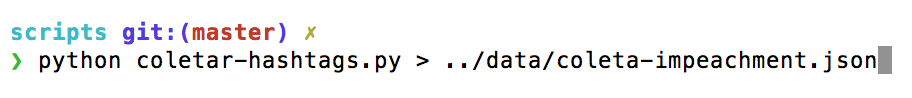
\includegraphics[width=0.95\textwidth]{Cap5/imagens/execucao-script}}
	\caption{Execução do \textit{script} para coleta de dados}
	\vspace{-0.3cm}
	\legend{FONTE: Elaborado pelo autor}
	\label{exec-coleta}
\end{figure}

O \textit{script} apresentado no Código~\ref{coleta-script} permaneceu em execução durante 14 horas (das 08:30 às 22:30) do dia 17 de abril, resultando em um arquivo de 2.6 gigabytes. O formato deste arquivo é um JSON, onde apresenta todas as informações presentes em um \textit{tweet}, como demonstrado através do Código~\ref{peda-json}.

\lstinputlisting[language=Python, label=peda-json, caption=Exemplo de um \textit{tweet} no formato JSON]{Cap5/src/peda.json}

\section{ANÁLISE DE DADOS}
Após a coleta dos dados foi gerado, então, um arquivo JSON de 2.6 gigabytes. Baseando-se nele, a etapa seguinte foi de analisar estes dados para extrair as informações consideradas úteis.

Foram realizados testes no arquivo JSON para verificar se existia algum tipo de \textit{dirty data}, que são informações quebradas, dados irrelevantes ou códigos que impedem a execução de \textit{scripts} de mineração \cite{dirty-data}. A Figura~\ref{fig-dirty} demonstra o único padrão de \textit{dirty data} encontrado dentro do arquivo.

\begin{figure}[h]
	\centering
	\fbox{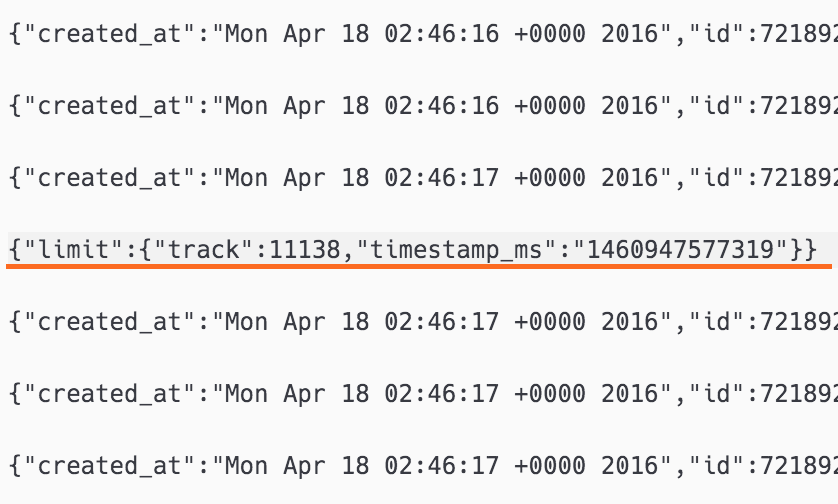
\includegraphics[width=0.95\textwidth]{Cap5/imagens/limit}}
	\caption{\textit{Dirty Data} presente no arquivo coletado}
	\vspace{-0.3cm}
	\legend{FONTE: Elaborado pelo autor}
	\label{fig-dirty}
\end{figure}

Dentro das milhares linhas do arquivo, existiam algumas linhas contendo este mesmo padrão ("limit":), que foram removidos utilizando outra ferramenta de sistemas baseados em Unix, o \textit{grep}.

A ferramenta \textit{grep} é considerada um "canivete suíço" \space para o uso de expressões regulares e possui uma funcionalidade que permite realizar uma consulta inversa, ou seja, o usuário passa um padrão ou uma palavra que deseja encontrar dentro de um determinado arquivo e, após encontrar todas as ocorrências, o \textit{grep} seleciona tudo o que não contém este padrão ou palavra.

Combinado com o comando de \textit{stdout} ($>$), é possível redirecionar todos os dados que não possui este tipo de \textit{dirty data} para um novo arquivo conforme a Figura~\ref{limpa-dado}.

\begin{figure}[h]
	\centering
	\fbox{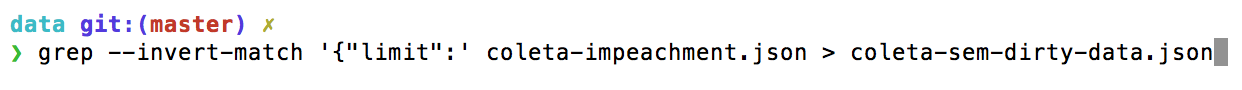
\includegraphics[width=0.95\textwidth]{Cap5/imagens/grep}}
	\caption{Utilizando o comando \textit{grep} para gerar um novo arquivo sem \textit{dirty data}}
	\vspace{-0.3cm}
	\legend{FONTE: Elaborado pelo autor}
	\label{limpa-dado}
\end{figure}

Após obter o arquivo JSON sem a presença de \textit{dirty data} foi possível iniciar o processo de extração de conhecimento utilizando o interpretador \textit{IPython}.

Nesta primeira etapa foram importados as bibliotecas necessárias para se trabalhar com arquivos do tipo JSON e também para a geração de gráficos, conforme o Código~\ref{ini-py}.

\lstinputlisting[language=Python, label=ini-py, caption=Leitura do arquivo JSON]{Cap5/src/ini.py}

A primeira linha do Código~\ref{ini-py} permite a visualização de gráficos e planilhas no \textit{IPython}. A partir da linha 8, é realizado a construção de um \textit{DataFrame}, definido na seção~\ref{pandas}, através leitura do arquivo coleta-sem-dirty-data.json.

A execução deste código permitiu, a geração um \textit{DataFrame} para informar o número de \textit{tweets} que ele contém. Esses \textit{DataFrames} possuem uma arquitetura semelhante ao formato de tabelas, em que é possível adicionar uma coluna ou uma tabela a uma variável em Python. \textbf{\textcolor{red}{[MELHORAR]}} Através do mapeamento de uma condição específica em um \textit{DataFrame}, apresentado no Código~\ref{map-lingua} para mapear o texto, a língua e o país em que o \textit{tweet} foi publicado.

\lstinputlisting[language=Python, label=map-lingua, caption=Mapeamento de variáveis para um \textit{DataFrame}]{Cap5/src/map-lingua.py}

Após o mapeamento das informações do \textit{DataFrame} foi construído um gráfico em barras indicando as quantidades de \textit{tweets} em relação aos quatro idiomas mais significativos no conjunto de dados coletados, Gráfico~\ref{lingua}.

\begin{grafico}[h]
	\centering
	\fbox{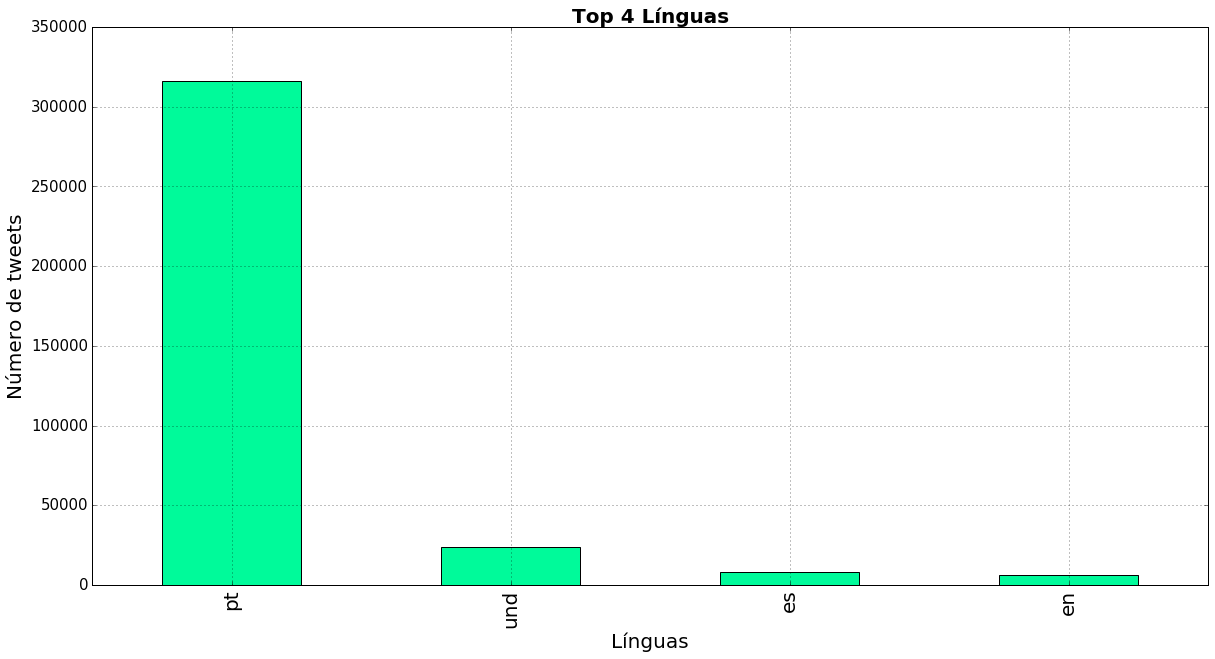
\includegraphics[width=1\textwidth]{Cap5/graficos/linguas}}
	\caption{Idiomas que mais realizaram \textit{tweets}}
	\vspace{-0.3cm}
	\legend{FONTE: Elaborado pelo autor}
	\label{lingua}
\end{grafico}

É possível verificar nesta figura que existe uma barra com o nome de \textit{und} para especificar o segundo idioma que mais realizou \textit{tweets}. Essa é uma condição em que não foi identificado o idioma de origem e, então, a API do \textit{Twitter} classifica como \textit{undefined}, ou indefinido no português. Essa linguagem indefinida ocorre devido ao \textit{software} em que o usuário está realizando o \textit{tweet}, por exemplo; um navegador \textit{web}, um aplicativo \textit{mobile} do \textit{Twitter} ou algum aplicativo de terceiro que permite realizar ações no \textit{Twitter}. Caso a linguagem não esteja definida nestes ambientes, a API a classifica como indefinida \cite{twitter-doc}.

Semelhante ao que foi realizado no Código~\ref{map-lingua}, através do Código~\ref{map-pais} foi possível verificar quais os países que estavam comentando sobre a \textit{hashtag} \#ImpeachmentDay através do Código~\ref{map-pais}.

\lstinputlisting[language=Python, label=map-pais, caption=Contabilização do número de \textit{tweets} por países]{Cap5/src/map-pais.py}

O Código~\ref{map-pais} verifica quais são os cinco países que mais realizaram \textit{tweets} através do mapeamento do \textit{DataFrame} e constrói um gráfico em barras para representá-los, Gráfico~\ref{paises}.

\begin{grafico}[h]
	\centering
	\fbox{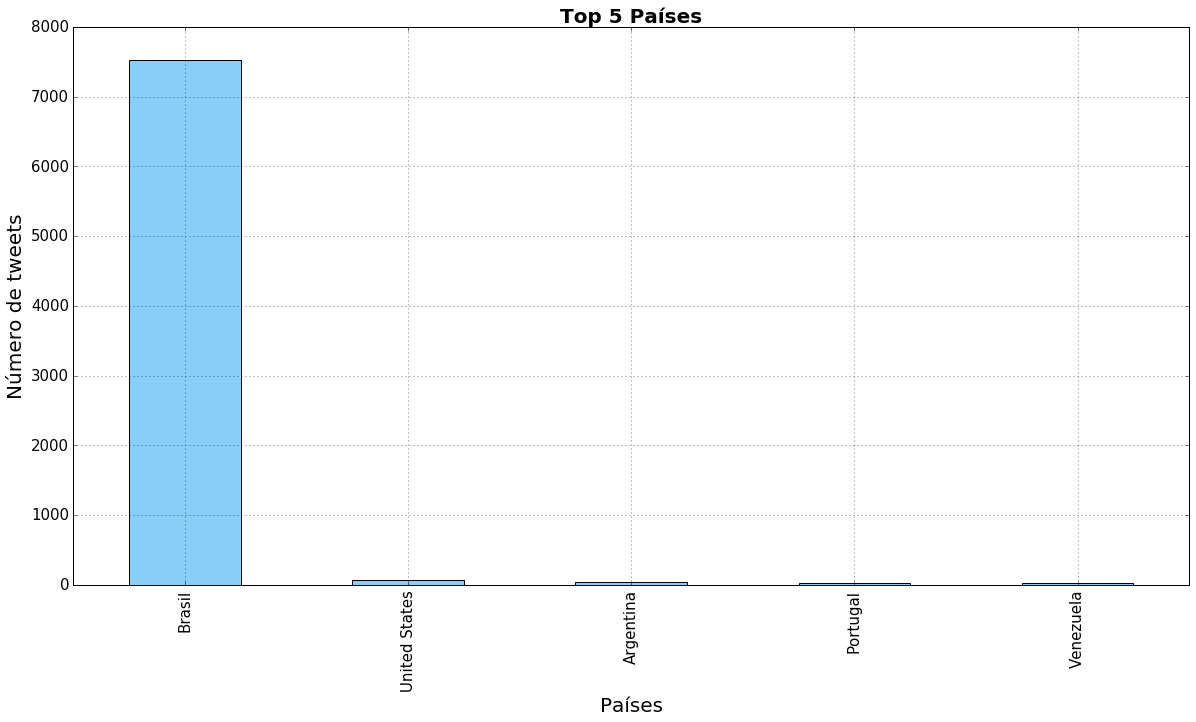
\includegraphics[width=1\textwidth]{Cap5/graficos/paises}}
	\caption{Países que mais realizaram \textit{tweets}}
	\vspace{-0.3cm}
	\legend{FONTE: Elaborado pelo autor}
	\label{paises}
\end{grafico}

Este gráfico demonstra, claramente, que a maior número de \textit{tweets} foram publicados do Brasil e apenas uma pequena quantia deles foram realizados nos Estados Unidos, Argentina, Portugal e Venezuela. É importante notar que nem todos os \textit{tweets} gerados possuem um país de origem, o que se assemelha a situação anterior, onde a API do \textit{Twitter} os classifica como \textit{undefined}, porém não sendo apresentado no gráfico da Figura~\ref{paises}.

Utilizando uma biblioteca para expressões regulares, é possível procurar por \textit{tweets} de palavras específicas, ou \textit{hashtags} mesmo o usuário digitando com letras maiúsculas ou minúsculas.

O Código~\ref{cod-hash}, apresenta uma função que procura determinadas palavras dentro do \textit{DataFrame}. Estas palavras então preenchem uma coluna com os \textit{tweets} relacionados com a palavra buscada. As palavras buscadas são referentes às \textit{hashtags} que mais foram publicadas nesta data.

\lstinputlisting[language=Python, label=cod-hash, caption=Buscar \textit{hashtags} mais publicadas]{Cap5/src/hashtags.py}

As \textit{hashtags} são contabilizadas e apresentadas através do gráfico de setores da Figura~\ref{hashtag}, onde é possível verificar a porcentagem referente aos \textit{tweets} realizados com a \textit{hashtag} \#ImpeachmentDay. 

\begin{grafico}[h]
	\centering
	\fbox{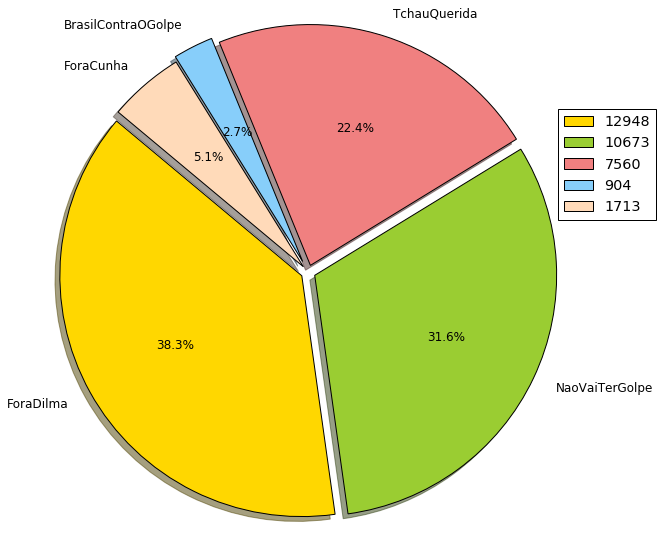
\includegraphics[width=1\textwidth]{Cap5/graficos/hashtag}}
	\caption{\textit{Hashtags} com o maior número de \textit{tweets}}
	\vspace{-0.3cm}
	\legend{FONTE: Elaborado pelo autor}
	\label{hashtag}
\end{grafico}

Através do Gráfico~\ref{hashtag}, pode-se notar que as \textit{hashtags} \#ForaDilma e \#TchauQuerida somaram um total de 60,7\%, indicando que a maioria dos \textit{tweets} eram de apoio ao processo de Impeachment da Presidente da República, diferentemente dos 34,3\% dos \textit{tweets} que é o somatório de \#BrasilContraOGolpe e \#NaoVaiTerGolpe.

Dando continuidade ao uso da biblioteca para trabalhar com expressões regulares, o Código~\ref{extract-link} permite encontrar \textit{links} que são publicados pelos usuários através de seus \textit{tweets}. Estes \textit{links} podem ser filtrados de acordo com a \textit{hashtag} utilizada.

\lstinputlisting[language=Python, label=extract-link, caption=Extração de \textit{links} provenientes de \textit{tweets}]{Cap5/src/extract-link.py}

\textbf{\textcolor{red}{[MELHORAR]}} O resultado da execução do Código~\ref{extract-link}, foi uma lista de milhares de \textit{links} e o número em ordem do \textit{tweet} encontrado no \textit{DataFrame}. A Figura~\ref{links} apresenta um pedaço desta lista para exemplificação.

\begin{figure}[h]
	\centering
	\fbox{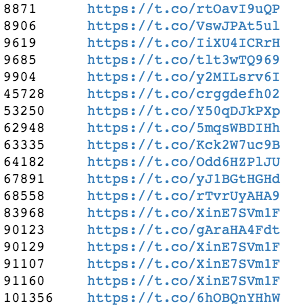
\includegraphics[width=0.5\textwidth]{Cap5/imagens/links}}
	\caption{Exemplo de \textit{links} extraídos de \textit{tweets}}
	\vspace{-0.3cm}
	\legend{FONTE: Elaborado pelo autor}
	\label{links}
\end{figure}

Semelhante ao Código~\ref{cod-hash}, é possível aplicar o filtro das \textit{hashtags} para encontrar nomes com maior popularidade através do Código~\ref{cod-fig-pol}.

\lstinputlisting[language=Python, label=cod-fig-pol, caption=Filtro para coletar nomes com mais \textit{tweets}]{Cap5/src/figuras-pol.py}

Como resultado, o Código~\ref{cod-fig-pol} constrói um gráfico em setores, onde é possível verificar a porcentagem de \textit{tweets} para nomes específicos, Gráfico~\ref{fig-pol}, porém não é possível, ainda, predizer se os argumentos a respeito destas pessoas são positivos ou negativos. \\

\begin{grafico}[h]
	\centering
	\fbox{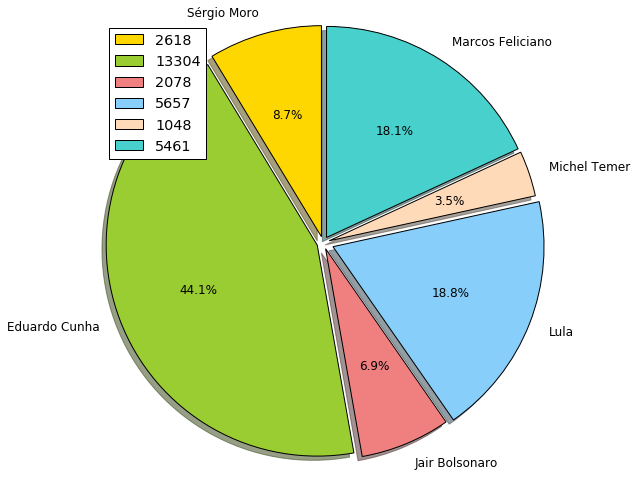
\includegraphics[width=1\textwidth]{Cap5/graficos/figuras-politicas}}
	\caption{Gráfico em setores para figuras importantes}
	\vspace{-0.3cm}
	\legend{FONTE: Elaborado pelo autor}
	\label{fig-pol}
\end{grafico}

O gráfico de setores representado pela Figura~\ref{fig-pol}, demonstra que o nome mais mencionado foi de Eduardo Cunha e com apenas 2618 \textit{tweets} o nome de Michel Temer foi publicado. Até mesmo as menções ao ex-presidente Luiz Inácio "Lula" da Silva recebeu apenas 18,8\% do total dos nomes filtrados.






























